\documentclass[a4paper, 11pt]{report}

%\usepackage{fullpage}



\usepackage[utf8]{inputenc} 
\usepackage[T1]{fontenc}
\usepackage{lmodern}
\usepackage{graphicx}
\usepackage[french]{babel}
\usepackage{color}
%\usepackage{fullpage}
\usepackage{array}
\usepackage[tight]{shorttoc}
\usepackage[toc,page]{appendix} 
\usepackage{makeidx} 
\usepackage{titlesec} % pour enlever "chapitre"


\definecolor{gris}{gray}{0.45}

\newcommand{\rouge}[1]{\textcolor{red}{#1}}
\newcommand{\rem}[1]{\textcolor{blue}{\emph{Remarque: \\} #1}}
\newcommand{\exl}[1]{\textcolor{gris}{\emph{Exemple: } #1}}
\newcommand{\exc}[1]{\textcolor{gris}{(\emph{Ex:} #1)}}
\newcommand{\cod}[1]{\textcolor{gris}{\emph{#1}}} 
\newcommand{\att}[1]{\textcolor{red}{\emph{\\ Attention: \\} #1 \\}}

\usepackage{listings}
\definecolor{dkgreen}{rgb}{0,0.6,0}
\definecolor{gray}{rgb}{0.5,0.5,0.5}
\definecolor{mauve}{rgb}{0.58,0,0.82}
\definecolor{red}{rgb}{1,0,0}

\newcommand{\lstconfig}[1]{
	\lstset{
	  language=#1,				      % the language of the code
	  basicstyle=\footnotesize,	      % the size of the fonts that are used for the code
	  numbers=left,				      % where to put the line-numbers
	  numberstyle=\footnotesize,	  % the size of the fonts that are used for the line-numbers
	  stepnumber=1,				      % the step between two line-numbers. If it's 1, each line 
									  % will be numbered
	  numbersep=5pt,				  % how far the line-numbers are from the code
	  backgroundcolor=\color{white},  % choose the background color. You must add \usepackage{color}
	  showspaces=false,			      % show spaces adding particular underscores
	  showstringspaces=false,		  % underline spaces within strings
	  showtabs=false,				  % show tabs within strings adding particular underscores
	  frame=single,				      % adds a frame around the code
	  tabsize=2,					  % sets default tabsize to 2 spaces
	  captionpos=b,				      % sets the caption-position to bottom
	  breaklines=true,				  % sets automatic line breaking
	  breakatwhitespace=false,		  % sets if automatic breaks should only happen at whitespace
	  title=\lstname,	   			  % show the filename of files included with \lstinputlisting;
									  % also try caption instead of title
	  numberstyle=\tiny\color{gray},  % line number style
	  keywordstyle=\color{blue},	  % keyword style
	  commentstyle=\color{dkgreen}\textit,   % comment style
	  stringstyle=\color{mauve}\textbf,	  % string literal style
	}
}
	
	\titleformat{\chapter}[hang]{\bf\huge}{\thechapter}{2pc}{} 
	\renewcommand{\appendixpagename}{Annexes}  
	\renewcommand{\appendixtocname}{Annexes}    
  

\begin{document}



\makeatletter
	\def\clap#1{\hbox to 0pt{\hss #1\hss}}%
	\def\ligne#1{%
	\hbox to \hsize{%
	\vbox{\centering #1}}}%
	\def\haut#1#2#3{%
	\hbox to \hsize{%
	\rlap{\vtop{\raggedright #1}}%
	\hss
	\clap{\vtop{\centering #2}}%
	\hss
	\llap{\vtop{\raggedleft #3}}}}%
	\def\bas#1#2#3{%
	\hbox to \hsize{%
	\rlap{\vbox{\raggedright #1}}%
	\hss
	\clap{\vbox{\centering #2}}%
	\hss
	\llap{\vbox{\raggedleft #3}}}}%
	\def\maketitle{%
	\thispagestyle{empty}\vbox to \vsize{%
	\haut{}{\@blurb}{}
	\vfill
	\vspace{1cm}
\begin{flushleft}
	%\usefont{OT1}{ptm}{m}{n}
	\huge \@title
\end{flushleft}
	\par
	\hrule height 4pt
	\par
\begin{flushright}
	%\usefont{OT1}{phv}{m}{n}
	\Large \@author
	\par
\end{flushright}
	\vspace{1cm}
	\vfill
	\vfill

\begin{center}
	
\includegraphics[width=5cm]{logo_UTBM.jpg}
\end{center}

\bas{}{Printemps 2013}{}
}%
\cleardoublepage
}
\def\date#1{\def\@date{#1}}
\def\author#1{\def\@author{#1}}
\def\title#1{\def\@title{#1}}
\def\location#1{\def\@location{#1}}
\def\blurb#1{\def\@blurb{#1}}
\date{\today}
\author{}
\title{}

% informations
\location{Belfort}\blurb{}
\makeatother
\title{Application des méthodes GOMS et Keystroke à la navigation vocale}
\author{\small{Paul \bsc{Locatelli} et Pierre \bsc{Rognon}}}
\blurb{%
	\textbf{GL40 - Interface homme/machine et perception}\\
	Université de Technologie de Belfort-Montbéliard
}% 


	
	\maketitle
	
	\newpage
	
	\shorttoc{Sommaire}{0}
	
	
	\chapter*{Introduction}
	\addcontentsline{toc}{chapter}{Introduction}
	
	Lors de ce semestre, des méthodes de calcul du temps nécessaire pour réaliser une tâche sur un ordinateur ont été étudiées. Ces calculs mettent en avant une comparaison afin de savoir dans quels cas un moyen est plus intéressant comparé à un autre. Cependant, lors de ces études, seuls deux moyens ont été étudiés: le clavier et la souris. Une troisième solution éventuelle était la combinaison des deux.\\ \ \\
	Cependant, si ces deux moyens sont généralement suffisant pour la vie de tous les jours afin de piloter un ordinateur de façon aisée, il convient de penser aux personnes pouvant éprouver des difficultés à l'utilisation de ces périphériques. Afin de palier à d'éventuels problèmes de mobilité des mains, qui peuvent empêcher d'utiliser de manière efficace la souris et le clavier, une solution peut-être la reconnaissance vocale afin de piloter un navigateur de fichiers par exemple.\\
	Le but de ce projet est donc de mettre en place des tests et l'interface nécessaire pour les réaliser afin de mesurer l'efficacité de cette troisième méthode. Ce rapport va donc détailler tout d'abord la composante de recherche vocale, puis se concentrer sur le navigateur et donc l'interface construite dans lequel les tests se dérouleront. Enfin, les fonctionnalités des tests en eux-même seront abordés ainsi qu'une synthèse sur l'efficacité de la méthode.
	
	\chapter{Analyse du projet}
	
	Afin de mieux formaliser les étapes qui doivent \^etre suivies tout au long du projet, il a été choisi de suivre ce qui a été appris lors de ce semestre en GL40. La première étape consiste donc à lister les différentes entités attenantes au sujet.\\
	
		\section{Liste des entités}
		
			\subsection{Liste des postes de travail}
			
			Un seul poste de travail est requis pour l'utilisation de l'application: le poste de l'utilisateur de celle-ci. Ce poste peut donc \^etre n'importe quel ordinateur ou machine capable de faire fonctionner le projet.
			
			\subsection{Liste des buts et sous-buts}
			
			Il n'y a qu'un but principal à cette application mais beaucoup d'autres en découlent. Ce principal but est \emph{le test de la méthode de navigation par la voix.}\\
			En découlent donc les sous-buts suivants:
			\begin{itemize}
				\item naviguer dans une arborescence de fichiers;
				\item éditer un fichier texte;
				\item lancer un test ou l'arr\^eter;
				\item consulter les résultats du test effectué.
			\end{itemize}
			
			\subsection{Liste des t\^aches et sous-t\^aches}
			
			Pour pouvoir réaliser les buts et sous-buts énoncés plus haut, des tâches sont requises. Les tâches principales sont:
			\begin{itemize}
				\item l'analyse des sons entendus;
				\item la recherche de l'arborescence à afficher;
				\item mesurer le temps lors d'un test.
			\end{itemize}
			
			Ces tâches sont aussi composées de sous-tâches:
			\begin{itemize}
				\item pour l'analyse des sons entendus:
				\begin{itemize}
					\item enregistrer le son;
					\item analyser le son;
					\item retourner le texte analysé.
				\end{itemize}
				\item pour le recherche de l'arborescence à afficher:
				\begin{itemize}
					\item parcourir le dossier en cours;
					\item retourner tous les fichiers et dossiers présents.
				\end{itemize}
				\item pour la mesure des temps lors d'un test:
				\begin{itemize}
					\item démarrer un timer lors du lancement du test;
					\item reconnaître la fin d'un test et arrêter le timer;
					\item calculer les temps attendus avec une autre méthode pour informer l'utilisateur.
				\end{itemize}
			\end{itemize}
			
			\subsection{Liste des données}
			
			
	
	\chapter{L'outil de reconnaissance vocale}
	
	Le développement d'un outil de reconnaissance vocale prenant énormément de temps, de ressources et demandant des connaissances solides dans le domaine, il aurait été impossible d'en développer au cours du projet. C'est pourquoi une recherche sur les modules de reconnaissance vocale a dû être effectuée. Ces logiciels n'étant pas très répandus et souvent propriétaires et payants, le choix n'a pas été aisé. Cependant, un module s'est détaché de tous les autres: Google Speech. Ce dernier est disponible dans plusieurs langues et sur de nombreuses plate forme ce qui en fait un outil flexible.\\
	Sa puissance réside surtout dans le fait que c'est un module exécuté sur des serveurs distants de la marque, qui sont efficaces.\\
	Cette puissance est donc aussi un inconvénient puisqu'elle implique une connexion effective avec les serveurs de Google lors de son utilisation. Le logiciel naissant de ce projet nécessitera donc un accès à internet permanent. N'ayant pas d'autre alternative crédible à la solution de Google, du fait d'une absence d'API pour les principaux concurrents (comme les modules de recherche vocale de Windows ou d'Ubuntu, qui s'ils sont efficaces ne sont pas utilisables dans un logiciel tiers), nous avons choisi Google Speech.\\ \ \\
	L'utilisation de Google Speech peut s'effectuer par l'intermédiaire d'un terminal (sous Linux ou Mac). Il n'y a pas de commande pour ce module à proprement parler mais Google Speech demande l'envoi du fichier audio où la reconnaissance vocale doit être appliquée. Une simple requête HTTP suffit donc pour l'utilisation du service. La solution la plus simple ici consistait donc à envoyer par l'intermédiaire d'un terminal le fichier audio enregistré à décoder. Le serveur Google Speech va se contenter alors de renvoyer le texte déchiffré.\\ \ \\
	Afin d'utiliser au mieux le service de Google, il a été choisi de segmenter un enregistrement permanent en fichiers audio de courte durée. Après quelques essais, il s'est avéré que 3 secondes étaient largement suffisantes pour les enregistrement puissent réunir une commande vocale entière sans qu'une partie de la commande soit sur un premier ficher et l'autre sur un second. Ce problème fait en effet échouer la reconnaissance puisqu'elle n'est alors pas pertinente.\\
	Le fait de devoir envoyer en permanence des informations afin de garder un enregistrement audio continu implique l'utilisation dans le projet de threads. Les threads permettent d'envoyer alternativement un fichier audio au serveur de Google et de continuer à enregistrer dans le même temps, ce qui évite des coupures.\\
	Lors des résultats sur les durées des tests passés dans le logiciel, il faudra donc prendre en compte le fait qu'une latence peut apparaître due à l'envoi des données au serveur Google, l'analyse de celles-ci et le retour vers la machine cliente.
	
	\chapter{L'interface logicielle}
	
	
	Afin de pouvoir réaliser des tests de calcul de la performance de la navigation vocale, il est nécessaire de mettre en place un support comportant des actions. Ces actions pourront \^etre chronométrées ou non pour laisser à l'utilisateur le choix d'utiliser le logiciel dans sa fonction secondaire utilisée pour le support. Cette fonction est un navigateur de fichiers avec visualisation de fichiers texte intégré. Ainsi, si l'utilisateur le souhaite, il peut naviguer dans ses fichiers et utiliser le logiciel comme un navigateur habituel. La différence ici est que le navigateur ne permet que de se déplacer dans l'arborescence de fichiers et d'ouvrir les fichiers dans l'éditeur intégré. L'utilisateur ne pourra donc pas ouvrir un fichier dans un autre logiciel. \\
	Malgré ceci, le but premier du projet étant de permettre la mise en place de tests chronométrés, il faut donc bien garder en t\^ete que le navigateur a pour fonction première d'\^etre un support aux tests.\\ \ \\	
	La matière étudiée pour ce projet se focalisant sur l'interface homme/machine, il est important d'attacher de l'importance à la composition de l'interface afin quelle soit utilisable aisément. C'est pourquoi il a été choisi de réaliser une interface simple, avec peu de boutons et répartis de manière astucieuse.\\
	Deux modes coexistent donc dans ce logiciel: un mode de navigation qui permet de se déplacer dans une arborescence de fichiers et un mode d'édition, réservée aux fichiers texte puisque c'est le seul utile aux tests, qui permet de lire, sélection, écrire et sauvegarder un fichier texte.
	
	\section{Le mode navigation}
	
	Le mode navigation est constitué de trois parties: la partie navigation "pure", la partie "boutons" et la partie "retour" de la reconnaissance vocale.\\
	
	\begin{center}
		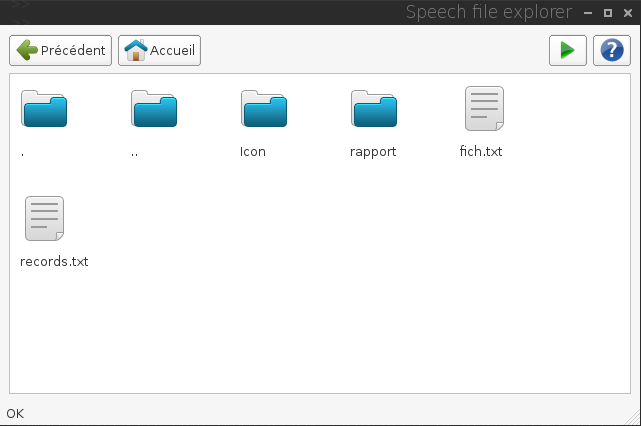
\includegraphics[width=11cm]{explorer}\\
		\emph{Ici, on peut voir l'interface lors du lancement du logiciel. Il ressemble à un navigateur de fichier standard simplifié.\\}
	\end{center}
	
	Comme dans tout navigateur de fichier, la plus grand partie de la fenêtre doit être affectée à la navigation de fichier. C'est pourquoi cette partie est insérée au centre afin d'attirer immédiatement l'attention de l'utilisateur. Les autres éléments doivent se faire suffisamment discrets pour ne pas perturber la concentration sur la navigation. Cependant, ils doivent être identifiables facilement et atteignable facilement.\\
	Les boutons ont donc été regroupés dans la partie haute de la fenêtre et divisés en deux parties: la partie aide à la navigation classique, la deuxième en lien avec notre but du projet, la navigation vocale.\\
	
	\begin{center}
		
\includegraphics[width=12cm]{buttons}\\
		\emph{La barre de boutons: à gauche les boutons d'aide à la navigation classique (accueil et précédent), à droite les outils pour la navigation vocale et les tests (lancer/arrêter le test, aide à la commande vocale).\\}
	\end{center}
	
	Le fait de diviser en deux les boutons permet de bien identifier les différentes fonctions du logiciel. La partie gauche existe sur la grande majorité des navigateurs de fichiers et sont placés au même endroit, l'utilisateur ne doit donc pas être perdu et l'ont ne cherche pas à bousculer cette règle. A droite, on peut se permettre de placer des fonctions spécifiques à notre logiciel puisqu'en lien avec le vocal.\\
	Le bouton "play", facilement identifiable de par son icône, lance un test. L'icône devient un carré rouge ensuite pour indiquer l'arrêt possible du test mais surtout qu'un test est en cours.\\
	Le bouton "aide", reconnaissable lui aussi permet d'ouvrir une fenêtre (voir ci-dessous) qui apporte une aide non négligeable pour un utilisateur non habitué du logiciel. On y indique les mots-clés reconnus par le logiciel pour la reconnaissance vocale. L'utilisateur peut s'y référer afin de mémoriser ces mots-clés.\\
	La partie du milieu de ce bandeau est laissée vide en temps normal, mais lors du pilotage à la voix, une interaction avec l'utilisateur est prévue; essayez donc de remercier le logiciel !
	
	\begin{center}
		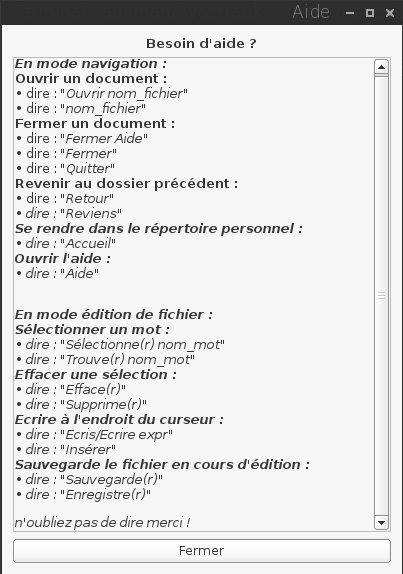
\includegraphics[width=8cm]{help}\\
		\emph{La fenêtre d'aide permet d'indiquer les mots-clés à utiliser pour la navigation par la voix à l'utilisateur.\\}
	\end{center}
	
	Le navigateur contient une troisième partie, tout en bas de la fenêtre, sur toute la longueur.\\
	Cette partie, très discrète puisqu'utile uniquement dans certains cas précis, a pour but d'indiquer ce que le logiciel reconnaît durant la reconnaissance.	On peut donc y voir la dernière interprétation renvoyée par Google Speech, qu'elle ait été interprétée correctement ou non.
	
	\section{Le mode édition}
	
	Ce second mode, nommé "édition", ne peut apparaître en démarrant le logiciel puisqu'il affiche le contenu d'un fichier. Ce mode est donc activé lorsque l'utilisateur, dans l'arborescence du navigateur, choisit non pas un dossier mais un fichier texte.\\
	Ici aussi, un intérêt a été porté au niveau de la simplicité de l'interface. Ainsi, pour ne pas dérouter l'utilisateur, la disposition reste la même: ni la barre de boutons, ni la partie de retour sur la reconnaissance ne changent de proportions. Et logiquement, l'édition étant le sujet principal de ce mode, il a été choisi de donner la plus grande partie de la fenêtre à l'espace édition et de centrer celui-ci. Ayant le même but pour la navigation, il a été choisi de simplement placer la surface d'édition à l'emplacement ou se trouve la partie navigation dans le mode du même nom. Ci-dessous, une capture du mode d'édition.\\
	
	\begin{center}
		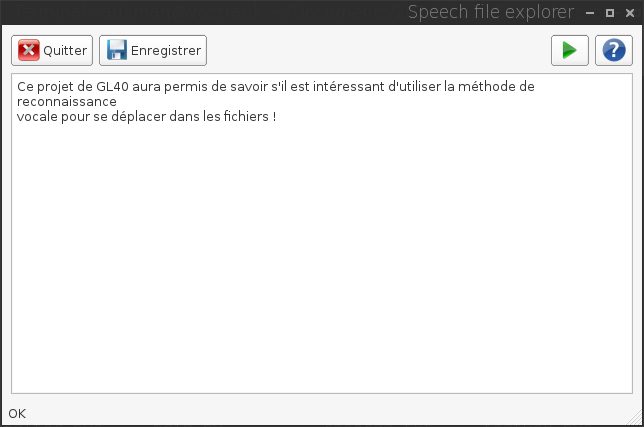
\includegraphics[width=10cm]{editor}\\
		\emph{Le mode édition est composé d'une partie édition prenant la majeure partie de la place, d'une partie boutons et d'une partie "retour". La proximité avec le mode navigation donne une cohérence au logiciel.\\}
	\end{center}
	
	
	La partie d'édition est très simple puisqu'il s'agit simplement d'une "boîte" où écrire du texte.\\
	Pour le bandeau de boutons, la partie de gauche évolue puisqu'elle est dédiée à la fonction principale actuelle qui est ici l'édition de fichiers et non plus la navigation. Les boutons donnent donc ici la possibilité de quitter le mode mais aussi de sauvegarder le fichier actuel pour ne pas perdre d'éventuelles modifications récentes. Des icônes ont été intégrées pour identifier plus facilement les actions en accord avec l'ensemble des boutons du logiciel.\\
	La partie inférieure de la fenêtre n'évolue pas par rapport au mode de navigation puisque la reconnaissance vocale a toujours lieu quelque soit le mode du logiciel.
	
	\chapter{Les tests d'efficacité}
	
	La partie la plus importante de ce projet puisque représentant son but premier est la partie de tests de la reconnaissance vocale. Malgré le fait qu'elle est l'objectif principal, il faut pour une utilisation la moins dérangeante possible que ces tests restent discrets. C'est pourquoi cette partie test est accessible à partir d'un simple bouton. Ce bouton à la façon d'un play/pause permet de lancer un test et de savoir lorsque celui-ci est terminé ou bien de l'arrêter.\\
	Deux tests ont été développés, en écho à ce qui a été étudié lors du semestre dans la matière: un premier test dans le navigateur qui a pour but de se rendre dans un fichier le plus rapidement. Le second test, dans l'éditeur, a pour but d'atteindre un certain endroit dans le fichier à partir d'un autre.
	
		\section{Le test du navigateur}
		
		Le test du navigateur a pour but de mesurer le temps que met l'utilisateur pour atteindre un fichier cible. Pour cela, il faut que le logiciel puisse enregistrer la cible à atteindre.\\
		Lorsque l'utilisateur veut lancer un test de navigateur, il faut donc qu'il clique sur le bouton de lancement de test. Cependant, pour que le test soit identifié, il faut en toute logique qu'il se situe en mode navigateur. C'est le fait qu'il soit en mode navigateur qui lance le bon test. Une fenêtre s'ouvre alors afin de recueillir les informations nécessaires (voir ci-dessous la fenêtre).\\
		
		\begin{center}
			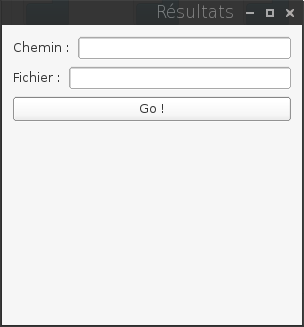
\includegraphics[width=5cm]{test}\\
			\emph{La fenêtre de test ci-dessus s'ouvre lorsqu'un test de navigateur est lancé.\\}
		\end{center}
		
		La fenêtre demande de remplir le chemin ainsi que le nom du fichier. Le chemin est simplement le dossier où le fichier est contenu. Cela permet d'éviter d'éventuelles erreurs de manipulation si l'on part d'un dossier où le même nom de fichier existant. Comme on ne vise pas ce dernier, il ne faut pas que le test s'arrête si l'on sélectionne ce fichier.\\
		Une fois les informations nécessaires renseignées, l'utilisateur lance le test. Ce test faire démarrer un chronomètre et on décompte donc le temps. Le lancement du chronomètre est visible par l'icône du bouton de test qui change (
\includegraphics[width=0.5cm]{stop}).\\
		La fenêtre reste cependant ouverte pour plusieurs raisons. Tout d'abord, cela permet de rappeler à l'utilisateur qu'un test est en cours en plus du changement d'icône dans le bouton de test. Cela permet aussi de pouvoir afficher une fois le test terminé les résultats. Afin d'indiquer à l'utilisateur qu'il n'a plus à entrer d'informations, on grise les champs comme le montre la capture ci-dessous.\\
		
		\begin{center}
			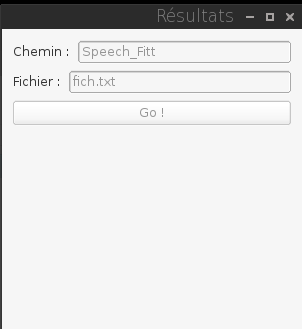
\includegraphics[width=5cm]{test_run}\\
			\emph{Une fois le test lancé, la fenêtre reste ouverte mais les champs sont grisés.\\}
		\end{center}
		
		Lorsque l'utilisateur arrive au fichier qui été visé, le test s'arrête automatiquement et les résultats sont instantanément affichée dans la fenêtre de test. Les résultats retournés sont affichés de la manière suivante:\\
		\begin{center}
			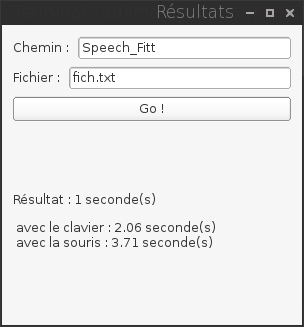
\includegraphics[width=5cm]{test_finished}\\
			\emph{Lorsque le test est terminé, on affiche les résultats dans l'encart prévu à cet effet.\\}
		\end{center}
		
		Le résultat obtenu lors du test effectif est comparé à des résultats calculés de manière théorique avec Keystroke. Cela permet à l'utilisateur de voir directement sa navigation a été plus efficace que le temps théorique.\\
	Cependant, si le but de ce test est de mesurer le temps mis par une navigation vocale, l'utilisateur devra s'imposer une discipline puisque le logiciel ne fait pas la différence entre clavier, souris ou voix. S'il veut réellement mesurer le temps de la navigation vocale, il devra donc lors du test ne pas "tricher". L'avantage est que la mesure au clavier ou à la souris sont possibles aussi. On peut alors comparer les temps réel mis par rapport au temps théorique.
	
	
		\section{Le test de l'éditeur}
		
		
	
	
	
	
	
	
		
	\newpage	
		
	\tableofcontents

		
\end{document}




